\chapter{Método de Trabajo}
\label{chap:metodo}

\drop{D}{urante} toda la extensión de este capítulo, se ahondará en las metodologías que se ha decidido seguir para la realización de este \acs{TFM}. En este caso, el marco de trabajo para la gestión de proyectos escogido ha sido Scrum, mientras que la metodología de desarrollo de software ha sido la del ciclo de vida iterativo e incremental.

\subsection{Motivación del uso de Scrum}
Esta metodología, al poseer artefactos como el \textit{Product Backlog} o eventos como el Sprint, junto con las reuniones diarias y las revisiones de los Sprints, se convierte en una de las mejores candidatas a aplicar a este trabajo. Por tanto, se ha realizado una interpretación de dicha metodología con el fin de poder adaptarla y adoptarla durante el desarrollo del \acs{TFM}.

\section{Scrum, una metodología de gestión de proyectos}
Scrum no se trata de una abreviatura de un término, sino de un concepto para la gestión de proyectos. Describe cómo un equipo puede implementar con mayor rapidez procesos complejos de desarrollo cuando el equipo se encuentra formado por pequeñas unidades auto-organizadas \cite{robertmulsow2018}. Se encuentra enfocado al uso de un proceso empírico que permite a los equipos responder con rapidez, eficiencia y eficacia al cambio \cite{michelesliger}. Dentro de este, es posible utilizar diferentes procesos y técnicas, dividiendo el proyecto en diferentes fases, de manera que una no puede comenzar si la anterior no ha finalizado \cite{scrumguide}.

\subsection{Pilares de Scrum}
Como se ha comentado anteriormente, se enfoca al uso de un proceso empírico (teoría de control de procesos empírica), obteniendo el conocimiento a partir de la experiencia adquirida de la toma de decisiones pasadas. Además, posee tres conceptos en torno a los que se desarrolla \cite{scrumguide}:

\begin{itemize}
    \item \textbf{Transparencia}. Esto representa que los aspectos importantes del proceso han de ser visibles a las personas que son responsables del resultado.
    \item \textbf{Inspección}. Este segundo concepto tiene que ver con la detección de desviaciones. Es decir, enfocándose en una meta concreta, los usuarios de Scrum han de revisar los artefactos que se vayan produciendo con el fin de detectar posibles variaciones no deseadas.
    \item \textbf{Adaptación}. No obstante, en el caso de que se haya producido alguna desviación indeseada, si un inspector determina que se han superado los límites aceptables, el proceso ha de ser reajustado lo más prontamente posible para evitar una desviación mayor.
\end{itemize}

\subsection{El marco de trabajo de Scrum}
Scrum provee una estructura para la entrega de resultados, no las prácticas específicas que se deben seguir, aspecto que se deja a libre elección. Por tanto, define un marco de trabajo que se muestra en la Figura \ref{fig:scrum_framework} \cite{scrumframewok}. A continuación, se procederá a detallar este marco, indicando los diferentes roles y responsabilidades que se pueden encontrar dentro de Scrum, así como los eventos y artefactos de los que se compone.

\begin{figure}[h]
  \centering
  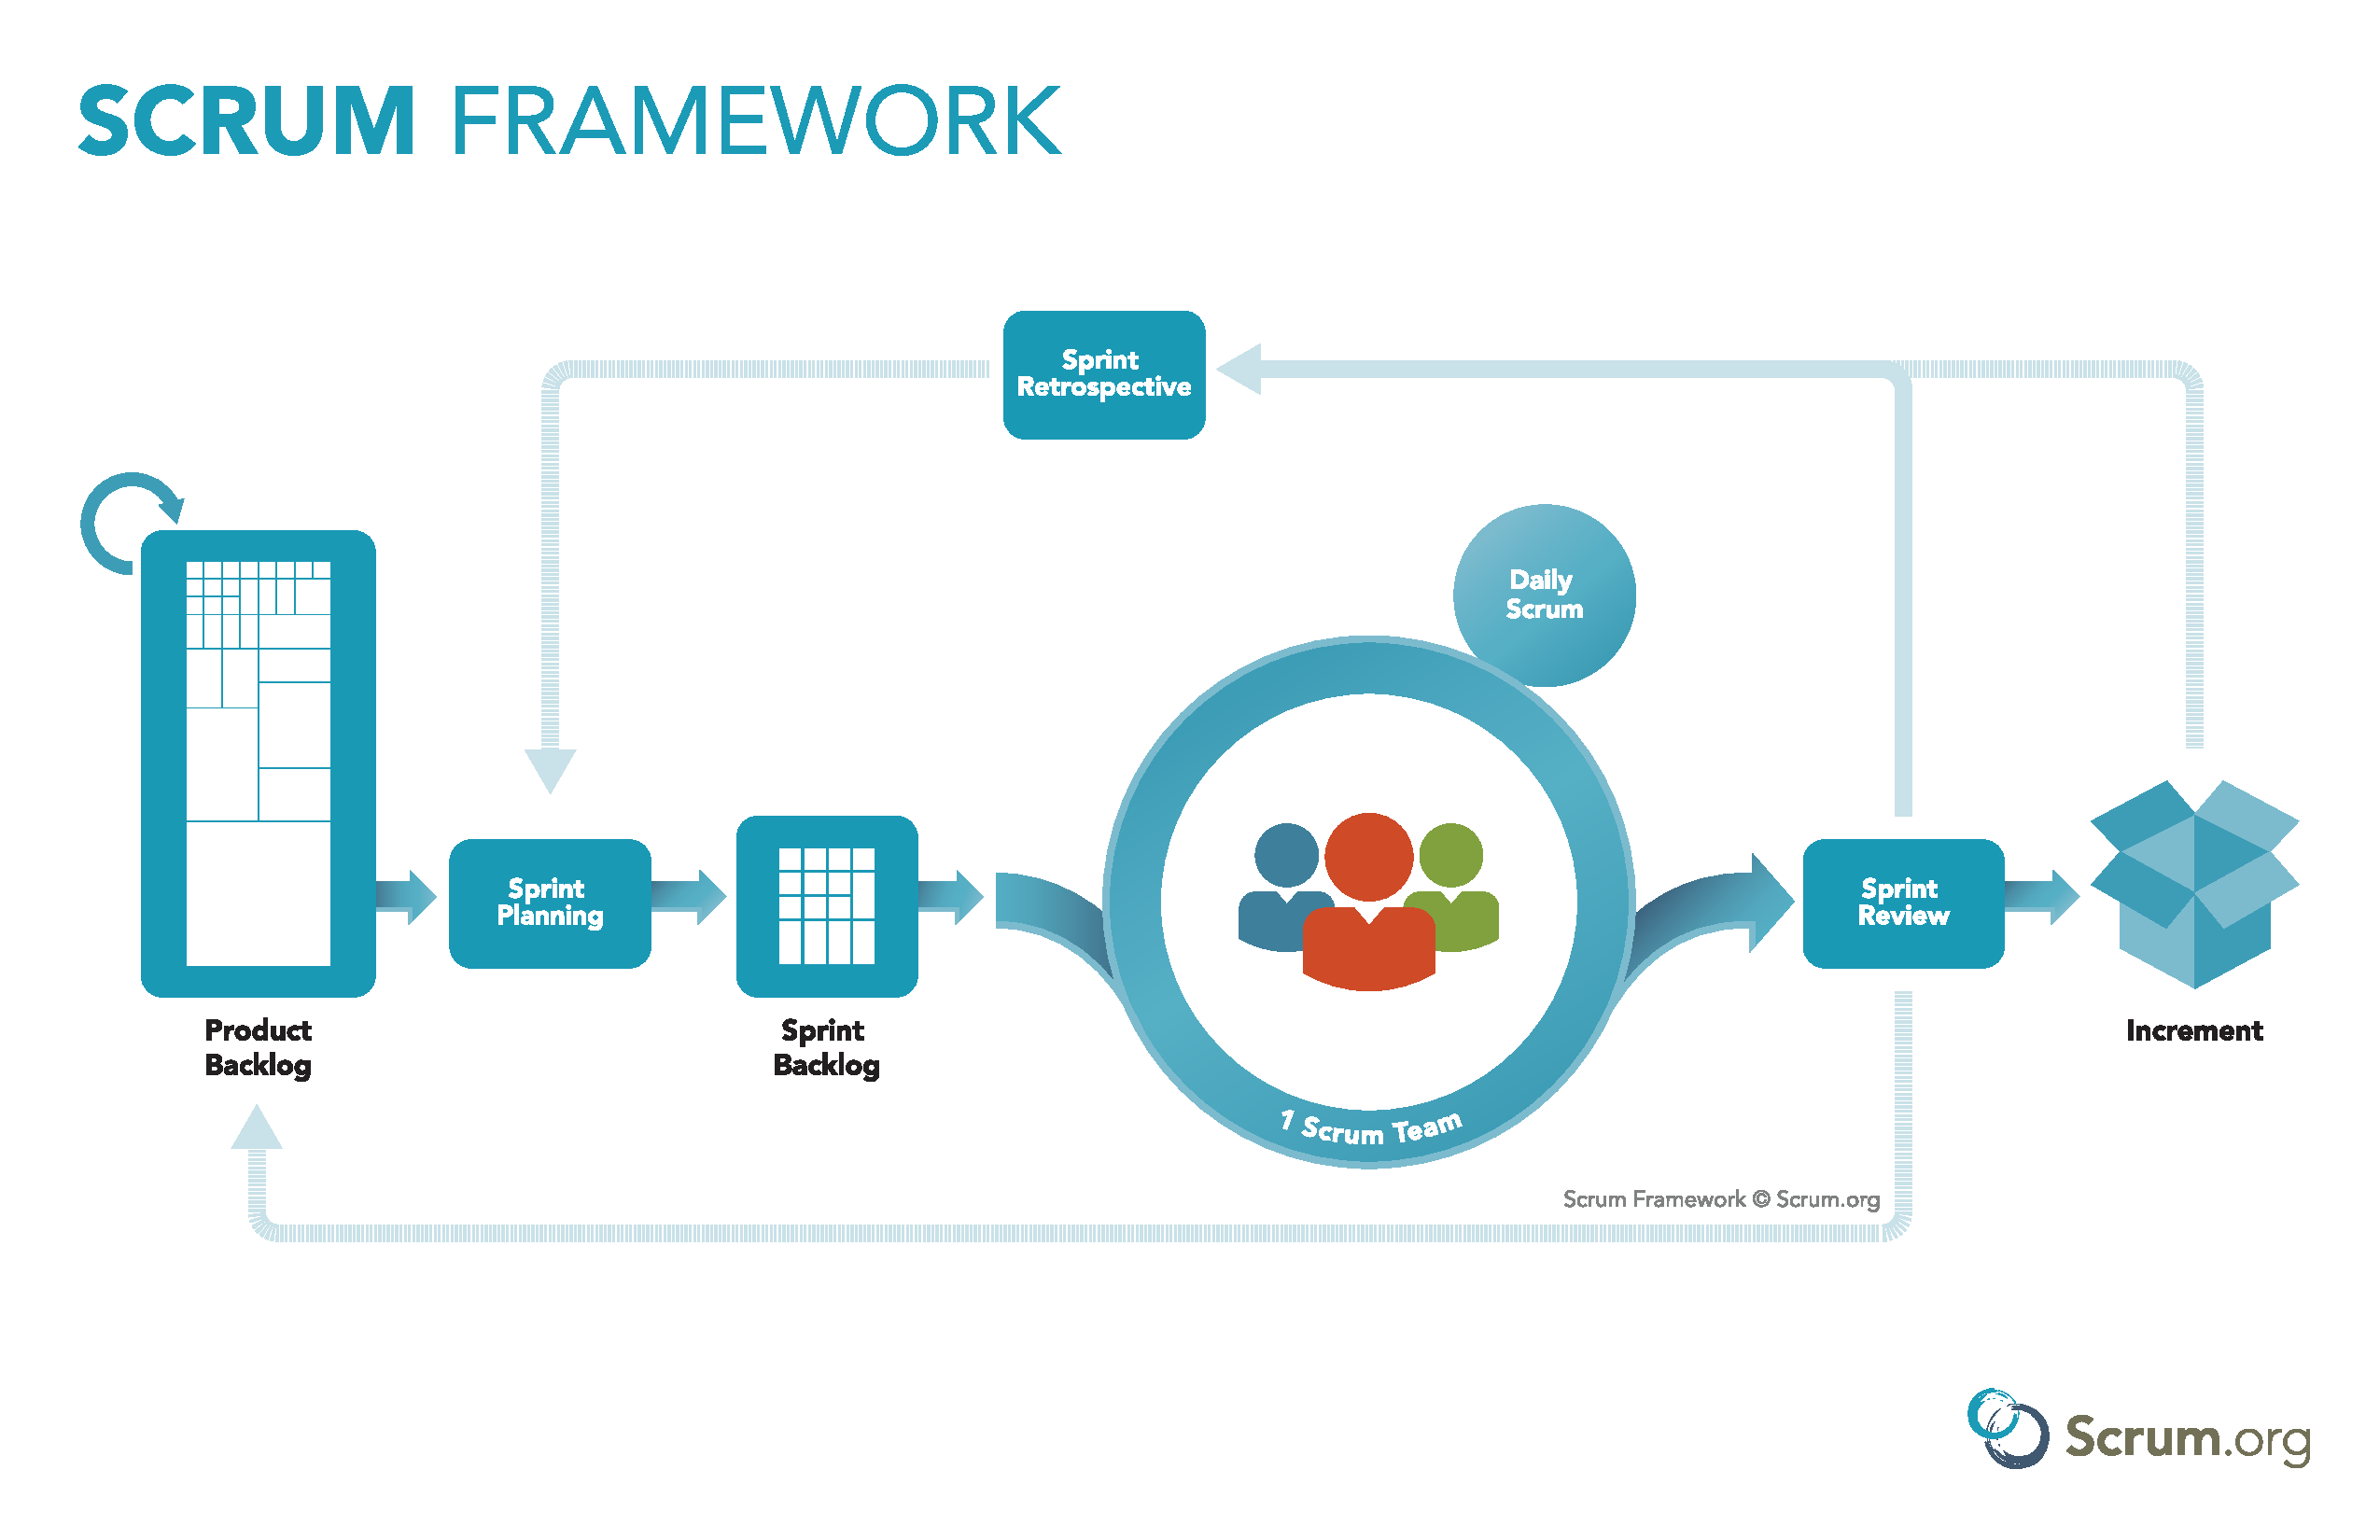
\includegraphics[width=0.8\linewidth]{figures/images/ScrumFramework.pdf}
  \caption{Marco de trabajo de Scrum}
  \source{\url{https://www.scrum.org/index.php/resources/scrum-framework-poster}}
  \label{fig:scrum_framework}
\end{figure}

\clearpage

\subsection{Roles y responsabilidades}
En Scrum existen tres roles principales: el Maestro de Scrum (\textit{Scrum Master}), el Dueño del Producto (\textit{Product Owner}) y el Equipo de Scrum (\textit{Scrum Team}).

\subsubsection{Maestro de Scrum (\textit{Scrum Master})}
Esta persona será la responsable de asegurar que todos los procesos se siguen correctamente, además de ejercer como defensor y protector del equipo ante amenazas o interferencias externas. Asegura y facilita la comunicación en el equipo, elimina obstáculos o media en las posibles discusiones que puedan aparecer. En definitiva, se trata de un <<facilitador>>.

\subsubsection{Dueño del Producto (\textit{Product Owner})}
Esta figura actúa en representación de los interesados (\textit{stakeholders}) del proyecto, siendo la voz de estos y con la capacidad de tomar decisiones sobre el producto. Realiza las funciones de mediador entre el equipo y el dueño del producto. Por otra parte, tiene el control sobre la Pila del Proyecto (\textit{Product Backlog}), por lo que también es el responsable de la definición, priorización o la correcta descripción de los elementos de los que esté compuesta.

\subsubsection{Equipo de Scrum (\textit{Scrum Team})}
Como regla general, el Equipo de Scrum ha de estar compuesto por siete más menos dos personas, que serán las encargadas de la entrega del producto y trabajarán sobre las diferentes tareas a realizar. Mientras que el Dueño del Producto se encarga del <<qué>>, el Equipo de Scrum se encarga del <<cómo>>. Su función última es la de entregar un incremento del producto terminado a final de cada Sprint. Las características más relevantes del Equipo de Scrum son las siguientes \cite{scrumguide}:

\begin{itemize}
    \item \textbf{Son autoorganizados}. La estructura y el modo de trabajo se conforman sin intervención externa explícita.
    \item \textbf{Son multifuncionales}. El conjunto de todos los miembros cuenta con las habilidades necesarias para desarrollar un incremento.
    \item \textbf{No se reconocen títulos individuales}. La responsabilidad de trabajo se asume por parte del equipo como unidad, es decir, el grupo es más importante que el individuo.
    \item \textbf{No se reconocen subequipos}. Este punto podría considerarse como una derivación del anterior, donde se indica que el grupo cuenta con mayor relevancia.
    \item \textbf{Cada miembro ha de tener habilidades especializadas y áreas en las que enfocarse}. Aunque es importante que cada miembro cuente con habilidades específicas, la responsabilidad final siempre recaerá sobre el conjunto del equipo.
\end{itemize}

\subsection{Eventos de Scrum}
Scrum se compone también de una serie de eventos que  se organizan en torno a bloques de tiempo o Sprints con el fin de crear un hábito y continuidad en el trabajo.

\subsubsection{El Sprint}
Este es el elemento principal en torno al que gira Scrum. Se trata de un bloque de tiempo con una duración fija y no superior a un mes dentro del que se desarrolla un entregable o incremento, no pudiendo dar comienzo al siguiente mientras el actual aún no ha terminado.


\subsubsection{Planificación del Sprint (\textit{Sprint Planning Meeting})}
Se trata de una reunión que se lleva a cabo en el primer día de cada Sprint con la finalidad de programar el trabajo a realizar durante el mismo y a la que atienden todos los roles de Scrum. En ella, el Dueño del Producto presenta todo lo que le gustaría ver completado y, entonces, el Equipo de Scrum determina las tareas a realizar. La reunión ha de finalizar con un \textit{Sprint Backlog}, un propósito para el Sprint, el compromiso del equipo y su estimación del esfuerzo requerido y la correcta comprensión de todas las tareas a realizar por parte de cada integrante.

\subsubsection{Scrum Diario (\textit{Daily Scrum})}
Este evento consta de una reunión de corta duración en la que se revisan las tareas realizadas, las que hay que realizar y se sincronizan las actividades, además de expone tanto lo que se ha realizado el día anterior como lo que se va a realizar en esa jornada y los impedimentos o problemas que pudieran haberse presentado. Con la intención de dotar al proyecto de una mayor agilidad, se ha optado por hacer uso de Microsoft Teams, donde se dispone de un canal con el mismo nombre dedicado a exponer todas esas cuestiones, obteniendo un \textit{feedback} cuando sea necesario.

\subsubsection{Revisión del Sprint (\textit{Sprint Review}) y Retrospectiva del Sprint (\textit{Sprint Retrospective})}
Este evento se trata de una reunión que se realiza al final de cada Sprint en la que el equipo convoca a los interesados para obtener \textit{feedback} a partir del entregable realizado. También, si fuera necesario, se ajustaría la Pila de Producto. Una vez que la revisión ha finalizado, el equipo lleva a cabo una retrospectiva con la finalidad de valorar el trabajo realizado durante el Sprint, de manera que se pueda crear un plan de mejora antes de la siguiente planificación.

\clearpage

\subsubsection{Aplicación de los eventos al \acs{TFM}}
Teniendo todo lo anterior en cuenta, para este trabajo se ha definido una duración de Sprint de dos semanas. No obstante, se desarrollará un primer Sprint denominado como Sprint 0 donde se fijarán los pilares del trabajo por lo que, teniendo en cuenta su naturaleza y el carácter del proyecto, como se expondrá más adelante, se definió la duración de este en una semana.

En cuanto al resto de eventos de Scrum, con el fin de poder adoptarlos en este proyecto, se han fijado reuniones todos los viernes con una duración estimada de alrededor de 45 minutos a las que se ha denominado como <<reuniones de seguimiento>>. Puesto que el Sprint tiene una duración de dos semanas, cada uno contendrá un total de dos reuniones, donde en una de ellas se realizará un seguimiento, mientras que la otra servirá para realizar la reunión relativa a la revisión del Sprint que acaba de finalizar, así como la planificación del próximo que vaya a comenzar.


\subsection{Artefactos de Scrum}
En Scrum, los llamados <<artefactos>> representan valor o trabajo y proporcionan transparencia a todas las personas implicadas en el proyecto. Estos artefactos se exponen a continuación \cite{scrumguide}.

\subsubsection{Pila del Producto (\textit{Product Backlog})}
Se trata de una lista ordenada en la que se incluye todo lo que va a ser necesario, y cuyo responsable es el Dueño del Producto. Es dinámica y suele estar sujeta a cambios, incluyendo las características, funciones, requisitos, mejoras y correcciones.

\subsubsection{Pila del Sprint (\textit{Sprint Backlog})}
Derivación del anterior artefacto, la Pila del Sprint se conforma a partir de la Pila del Producto y contiene todos los trabajos que se han de realizar en un determinado Sprint. De igual manera, es dinámica y se va modificando conforme avanza el Sprint.

\subsubsection{Incremento}
El incremento es la suma de todos los elementos que se han completado en el Sprint y el valor que aportan los Sprints anteriores.

\subsubsection{Aplicación de los artefactos al \acs{TFM}}
En cuanto a la adopción de los artefactos de Scrum, tanto para la Pila del Producto como para la Pila del Sprint se hará uso de Microsoft Planner, moviendo las tareas de la Pila de Producto al correspondiente bloque del Sprint, como se detallará en mayor profundidad en una sección posterior de este capítulo.



\clearpage

\section{Ciclo de vida iterativo e incremental}
Este ciclo de vida se encuentra ligado a Scrum por tratarse de una metodología ágil y consiste en el desarrollo por partes del producto, integrando estas partes de manera progresiva conforme se van completando. Conforma una de las bases de un proyecto ágil puesto que se cuenta con iteraciones cortas en el tiempo \cite{javiergarzas2012}, de manera que el producto final va adquiriendo una mayor funcionalidad y, por tanto, una mayor calidad final. Por otra parte, en cada iteración se revisa y mejora el producto, añadiendo nuevos requisitos o mejorando los ya existentes \cite{proyectosagiles}. En cierto modo, se crean proyectos más pequeños entre los que se reparte el trabajo total donde cada uno representa una iteración que generará un incremento como resultado. Todos estos proyectos derivados siguen el esquema análisis-diseño-pruebas (Figura \ref{fig:iteraincr}), así como serie de ventajas: el riesgo del proyecto se ve acotado a un incremento, permite concentrar el esfuerzo de los desarrolladores para mejorar la eficiencia en cada iteración y se puede conseguir una mejor especificación de los requisitos.

\begin{figure}[h]
  \centering
  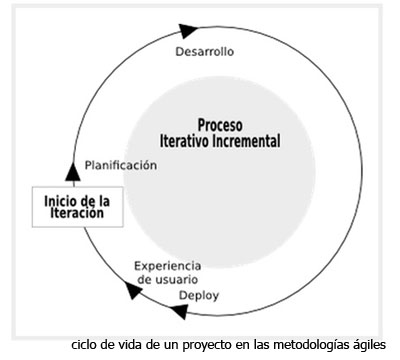
\includegraphics[width=0.52\linewidth]{figures/images/ciclo_iterativo_incremental.jpg}
  \caption{Ciclo Iterativo e Incremental}
  \source{\url{https://commons.wikimedia.org/wiki/File:Ciclo_de_vida_proyecto_metodologia_agiles.jpg}}
  \label{fig:iteraincr}
\end{figure}

\clearpage

\section{Recursos}
La realización de este trabajo no requiere de hardware especial ni específico más allá de disponer del sistema operativo Windows debido al uso de los servicios de Azure. El software, por otra parte, sí que debe estar dotado de ciertas características específicas debido al uso de determinadas herramientas.

\subsection{Recursos hardware}
Principalmente, debido a la necesidad de utilizar el sistema operativo Windows, se ha utilizado un ordenador con la versión de Windows 10 Home, en su versión de compilación 1903.

\subsection{Recursos software}
Puesto que la metodología escogida ha sido Scrum y esta posee una serie de eventos que deben producirse a lo largo del desarrollo del proyecto, se hará uso de software que permita seguir adecuadamente dicha metodología. Por otra parte, también se expondrá otro software que, si bien no es relativo a la metodología, se deberá utilizar para cumplir con los objetivos definidos.

\subsubsection{Microsoft Teams}
Microsoft Teams \cite{microsoftteams} es una aplicación multiplataforma cuyo fin es el de coordinar el trabajo y favorecer la comunicación de los integrantes de los grupos dentro de una empresa. Ofrece diferentes funcionalidades, que tienen que ver con lo relacionado con las reuniones, llamadas, dispositivos, mensajería instantánea o la capacidad de integración con otras aplicaciones. Este software permite realizar conferencias de audio, vídeo y web con personas de dentro y fuera de la organización, así como proporcionar asistencia, tomar notas, compartir el escritorio o cargar archivos. Para este tipo de reuniones, en el caso de ser numerosas, Microsoft Teams cuenta con la capacidad de retransmitirlas en directo con hasta 10.000 asistentes. Por otra parte, también es posible unirse a reuniones desde un teléfono convencional o usar Microsoft Teams para llamar a una persona directamente sin necesidad de Internet.

No obstante, principalmente, en el desarrollo de este trabajo, se hará uso de todo lo relacionado con la mensajería instantánea y la integración de aplicaciones con objeto de seguir la metodología y en pos de llevar una coordinación. Es posible definir equipos de trabajo con diferentes canales según su propósito. En cada uno de estos canales es posible la comunicación entre todos los miembros del equipo, así como adjuntar archivos, imágenes o vídeos utilizando texto enriquecido. Además, es posible enlazar e integrar dentro del mismo software otras aplicaciones como la suite ofimática de Microsoft Office 365, Microsoft Planner o aplicaciones de terceros como MindMeister, de las que se hablará a continuación.

\subsubsection{Microsoft Planner}
Este software \cite{microsoftplanner} permite la organización del trabajo dividido por tareas y <<depósitos>> o bloques. Se inspira en la filosofía de los tableros Kanban, por lo que es más fácil organizar el trabajo de una manera más visual. Además, cada una de las tareas cuenta con un mayor nivel de detalle, como la asignación de esta a una persona del equipo, establecer la importancia mediante el uso de etiquetas, añadir una pequeña descripción o indicar un comentario. Por otra parte, aporta información visual en forma de gráficos, de manera que se pueda llevar un seguimiento de las tareas realizadas, en curso y las no comenzadas, por lo que este recurso será de utilidad, sobre todo, para la aplicación de la metodología escogida.

No obstante, aunque Planner no se encuentra diseñado inicialmente para trabajar con Scrum, es posible su adaptación \cite{robertmulsow2018} mediante la creación de diferentes bloques, donde cada uno representará un Sprint y cada tarea, un elemento del \textit{Product Backlog}. Además, todas las tareas se podrán detallar en mayor medida dependiendo de la criticidad (crítico, importante, normal, bajo), asignación a los integrantes del grupo, descripción o el estado en el que se encuentra en cada momento, así como recursos gráficos que ayuden a comprender el grado de desarrollo del proyecto.

\subsubsection{MindMeister}
MindMeister \cite{mindmeister} es un software online dedicado a la creación de mapas mentales colaborativos, permitiendo plasmar y compartir ideas de forma gráfica. Sobre todo, es apropiado para las lluvias de ideas, tomar notas o planificar proyectos colaborando con los integrantes del equipo. Por tanto, resultará de utilidad en el caso de que se deseen plasmar de manera rápida pero ordenada algunas ideas que, por ejemplo, puedan surgir en las reuniones o durante el desarrollo del proyecto, además de construir el mapa mental del \acs{TFM} de manera iterativa.

\subsubsection{Microsoft OneNote}
Microsoft OneNote \cite{onenote} es una aplicación multiplataforma que permite tomar notas como si un bloc de notas se tratase, con una ordenación por libros, secciones y páginas. Además, en el caso de usarse en un dispositivo móvil, ofrece la capacidad de dibujar o escribir con el dedo o con un lápiz, lo que será ayudará a la hora de recoger todo de lo que se trate en las diferentes reuniones que se lleven a cabo durante el desarrollo del proyecto. Todos estas anotaciones se sincronizarán con la nube de Azure y podrán ser vistas por todos los integrantes en tiempo real, estando disponibles para su consulta desde la aplicación móvil, web o su integración con Microsoft Teams. Será de utilidad en este trabajo a la hora de tomar notas durante las reuniones y llevar un seguimiento de los temas tratados durante las mismas, de manera que se pueda recurrir a estas una vez finalizadas.

\subsubsection{\textit{Balsamiq Mockups}}
\textit{Balsamiq Mockups} \cite{balsamiq} se trata de una herramienta para el prototipado de interfaces gráficas de aplicaciones a través de la realización de bocetos por ordenador. Permite plasmar de una manera rápida y ágil la idea que se tiene acerca de cómo se entregará al usuario final una aplicación, haciendo posible disponer de un apoyo a la hora de llevar a cabo el desarrollo de los diferentes programas. Ofrece todos los elementos de los que se puede componer una interfaz gráfica como botones, listas desplegables, cuadros de texto o etiquetas con un método de trabajo sencillo de comprender. Además, es posible trabajar con flujos de interacción dentro de los propios bocetos, insertando enlaces en los botones para emular los eventos que podrían suceder en la aplicación real, lo que lo hace muy apropiado cuando se trata de obtener un \textit{feedback} del usuario para implementar mejoras o modificaciones. Por tanto, esta herramienta será de utilidad en el desarrollo de la interfaz gráfica de la aplicación de gestión, ya que se podrá validar su apariencia y funcionalidad asociada antes de que den comienzo las tareas de programación.

\subsubsection{Microsoft \textit{Visual Studio}}
\textit{Visual Studio} \cite{visualstudio} es una herramienta de Microsoft que se encuentra dentro de la categoría de \acf{IDE}, o Entorno de Desarrollo Integrado, en español. Entre sus funcionalidades principales se encuentra la integración con otros servicios como Azure o GitHub, compatibilidad con el desarrollo de aplicaciones web o la capacidad de desarrollar aplicaciones basadas en C++, C\# o \acf{VB}. Por otra parte, también provee facilidades enfocadas tanto a las labores de programación como a las de análisis, depuración, pruebas o colaboración. Esta herramienta se convierte en una de las imprescindibles cuando se trata de desarrollar aplicaciones para \acf{UWP}, por lo que será utilizada en el desarrollo de la interfaz gráfica de usuario de la solución para la administración del servicio de \acf{WVD}.

\clearpage

\subsection{Recursos \textit{cloud}}
Este bloque se encuentra dedicado a exponer los recursos \textit{cloud} de los que se hará uso puesto que no pertenecen de manera estricta al conjunto anterior de recursos software.

\subsubsection{Microsoft Azure}
Azure \cite{queesazure} es el nombre que recibe la plataforma de servicios de informática en la nube, de pago por uso, de la empresa Microsoft. Atendiendo a los niveles \textit{cloud} tradicionales, proporciona servicios tanto de infraestructura como de plataforma (\acs{IaaS} y \acs{PaaS}). Es posible seleccionar el software que se desea de entre los que se encuentran disponibles en su catálogo, así como escalar los recursos de manera casi instantánea según las necesidades, facturando únicamente por lo que se está utilizando. Al igual que otras plataformas que ofrecen estos servicios, ofrece una mayor seguridad y productividad que las soluciones \textit{on-premise}, ayudando a desarrollar la actividad de las empresas de una manera más eficiente. Por otra parte, dispone de centros de datos en numerosas regiones, lo que permite operar reduciendo costes, tiempo de acceso y respuesta y distancia con respecto al lugar geográfico de operación del cliente.

Este recurso tendrá una gran importancia en este trabajo, puesto que será clave e imprescindible para llevar a cabo la implementación del servicio que se plantea desarrollar debido a que, desde esta plataforma, se tiene acceso a uno de los servicios que ofrece y que se explica en la siguiente sección.

\subsubsection{\acf{WVD}}
Windows Virtual Desktop es una solución que presentó Microsoft a finales del pasado año 2018 como un servicio dentro de Azure que permitía virtualizar escritorios y aplicaciones. Se lanzó en versión preliminar privada en septiembre y actualmente ya se encuentra en versión preliminar pública desde marzo de este año, estando previsto que salga de esta fase a finales de año \cite{juliawhitebradanderson2019}. Este servicio será el núcleo del \acs{TFM}, ya que el modelo de negocio girará en torno a este, aprovechando el potencial y las funcionalidades que ofrece a la hora de entregar tanto aplicaciones virtualizadas como escritorios remotos completos. Algunas de las funcionalidades que ofrece son las siguientes \cite{microsoftwvd2019}:

\begin{itemize}
    \item Configurar una implementación de Windows 10 multisesión que proporcione escalabilidad.
    \item Virtualizar Office 365 ProPlus y optimizarlo para su ejecución en \mbox{escenarios} virtuales multiusuario.
    \item Proporcionar escritorios virtuales de Windows 7 con actualizaciones de seguridad ampliadas gratuitas hasta enero de 2023.
    
    \clearpage
    
    \item Proporcionar y migrar los servicios \acf{RDS} existentes, escritorios de Windows Server y aplicaciones en cualquier ordenador.
    \item Virtualización de escritorio y aplicaciones.
    \item Gestionar escritorios de Windows 10, Windows Server y Windows 7 y aplicaciones con una experiencia unificada de gestión.
\end{itemize}

\subsection{Recursos metodológicos}
En este trabajo, aparte de los recursos hardware y software especificados, se utilizarán también otros recursos que no se pueden clasificar dentro de esas dos categorías y que se detallan a continuación.

\subsubsection{Análisis PESTEL}
Se trata de un acrónimo \cite{juanmartin2017} y consiste en llevar a cabo un análisis teniendo en cuenta diferentes contextos o dimensiones: política, económica, socio-cultural, tecnológica, ecológica y legal (Figura \ref{fig:pestel}). Su objetivo es el de identificar variables de impacto dentro de un ámbito territorial clasificándolas por las dimensiones y calificadas con un determinado nivel de impacto. Este análisis se caracteriza por ser adaptable a cada caso, proporciona ayuda en la toma de decisiones, posee un enfoque proactivo y es de aplicación amplia, anticipando cambios y vislumbrando tendencias. Por tanto, será de utilidad a la hora de realizar el análisis del entorno general de operación para obtener una descripción del contexto externo en el que se encontrará la actividad de la empresa.

\begin{figure}[h]
  \centering
  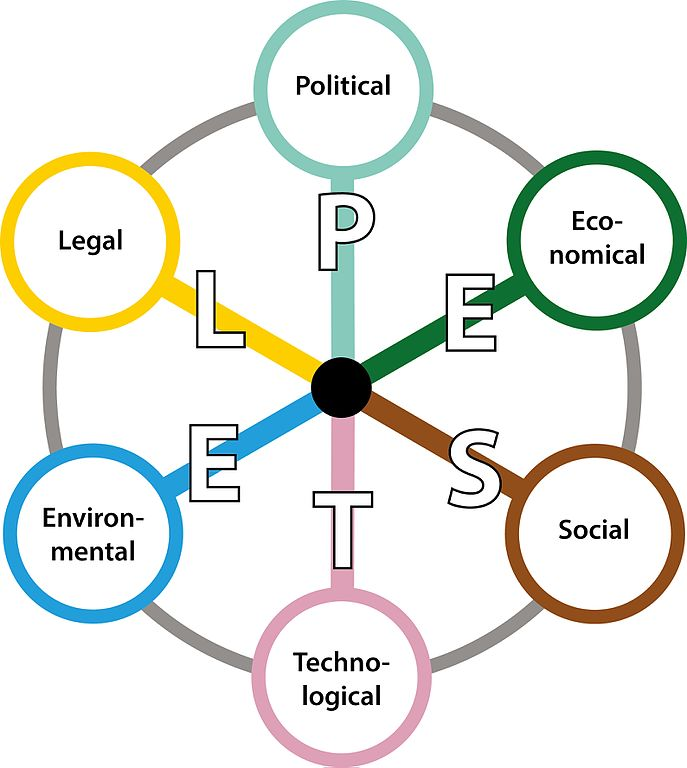
\includegraphics[width=0.45\linewidth]{figures/images/PESTEL.jpg}
  \caption{Dimensiones del análisis PESTEL}
  \label{fig:pestel}
\end{figure}

\clearpage

\subsubsection{Análisis de las 5 fuerzas de Porter}
Este análisis fue propuesto por Michael Porter \cite{Porter1989HowStrategy}, de la Universidad de Harvard, en un artículo que data del año 1979. Proporciona un marco de reflexión estratégica en el que se identifican unas determinadas fuerzas o influencias externas dentro del entorno específico de operación que pueden afectar al desarrollo de la actividad empresarial. Estas fuerzas se representan en la Figura \ref{fig:fuerzas_porter} y son las que pueden ejercer tanto los proveedores como los clientes o la rivalidad que pueda existir entre los competidores existentes, así como las amenazas de entrada que pueden ejercer los potenciales competidores y la de los productos sustitutivos. Por tanto, se trata de una herramienta especialmente estratégica que se utiliza con el fin de elaborar planes estratégicos y modelos de negocio \cite{josemanuel}. Por tanto, este análisis resulta complementario para el análisis PESTEL puesto que, realizando ambos, se consiguen focalizar los aspectos analizados a una industria específica sin perder de vista el entorno general donde va a operar la empresa, ayudando en la toma de decisiones posterior.

\begin{figure}[h]
  \centering
  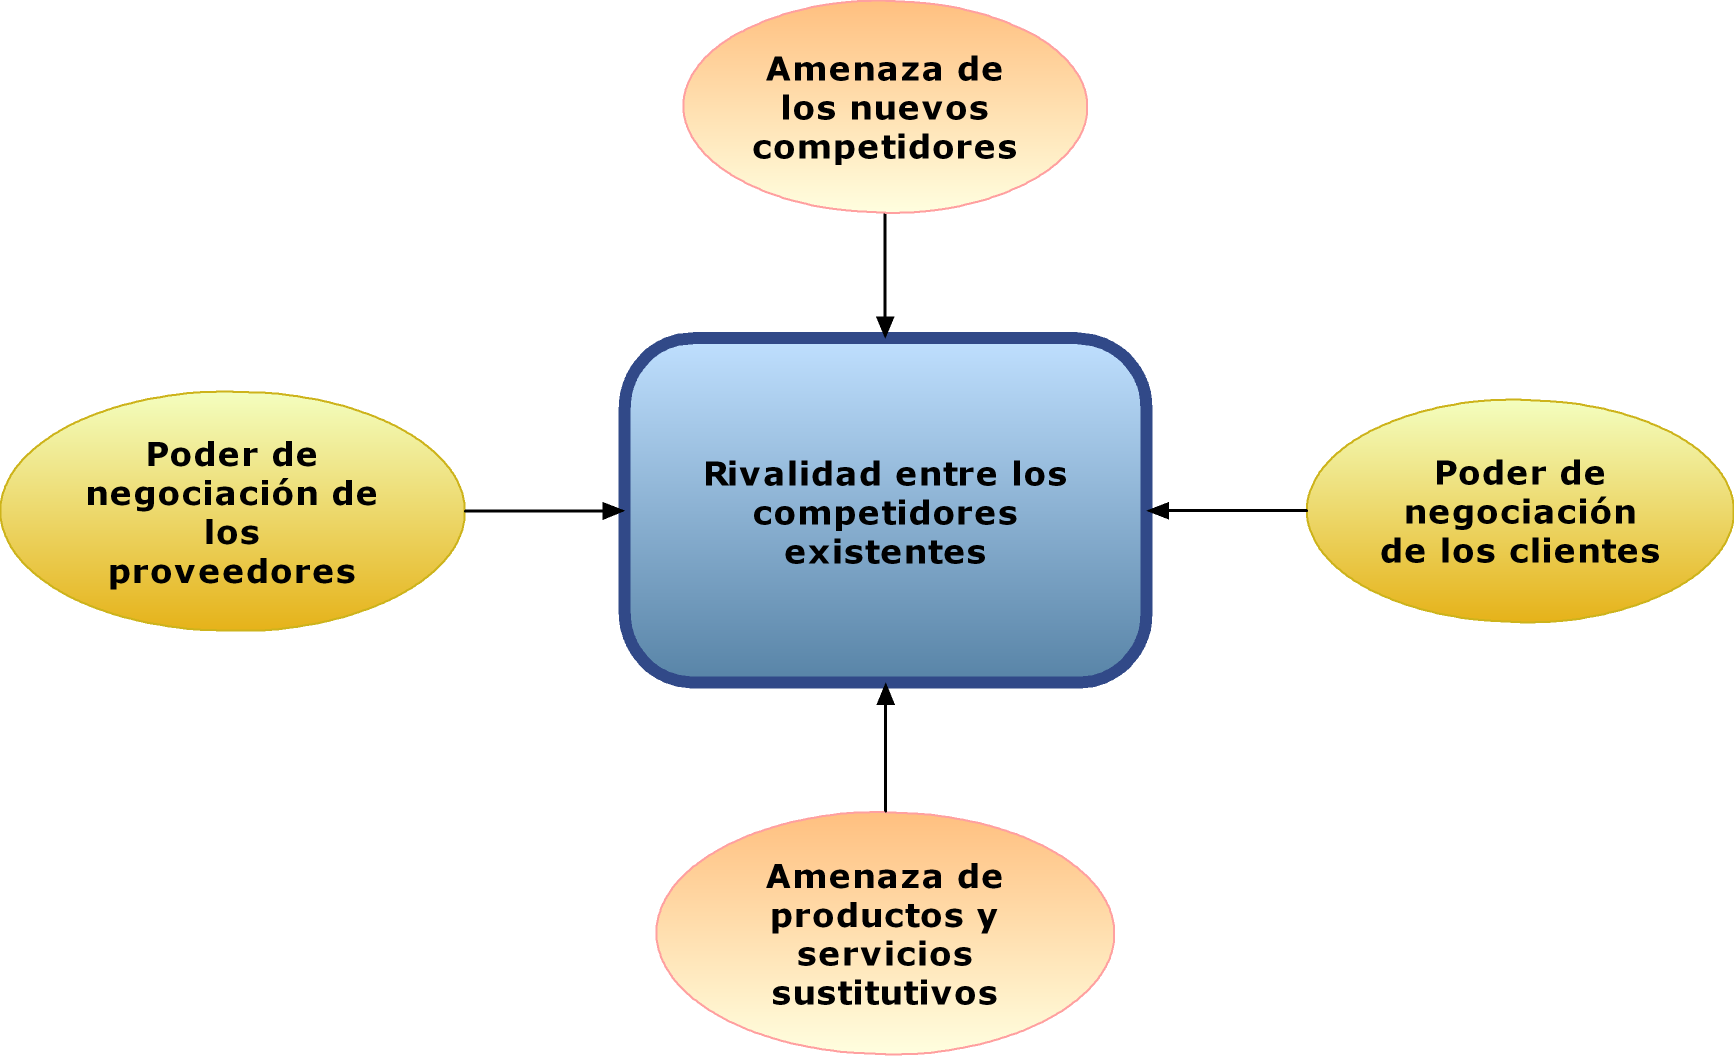
\includegraphics[width=0.75\linewidth]{figures/images/Modelo_Porter.png}
  \caption{Modelo de Porter}
  \label{fig:fuerzas_porter}
\end{figure}

\clearpage

\subsubsection{Lienzo del Modelo de Negocio (\textit{Business Model Canvas})}
Esta herramienta \cite{cristinaramosvega2018} fue diseñada por Alexander Osterwalder junto con Yves Pigneur y permite definir y categorizar los diferentes elementos de una empresa con respecto a la definición de su modelo de negocio una vez se han tenido en cuenta tanto el entorno general como el específico, pues permite establecer y mantener ordenados diferentes elementos que poseen una cierta relevancia dentro de este. Esencialmente, se trata de un <<lienzo>> que permite observar de un vistazo el modelo de negocio de una empresa y se compone de nueve bloques diferenciados donde se tienen en cuenta los clientes, lo que ofrece la empresa, la infraestructura y la viabilidad económica (Figura \ref{fig:bmc}).

\begin{figure}[h]
  \centering
  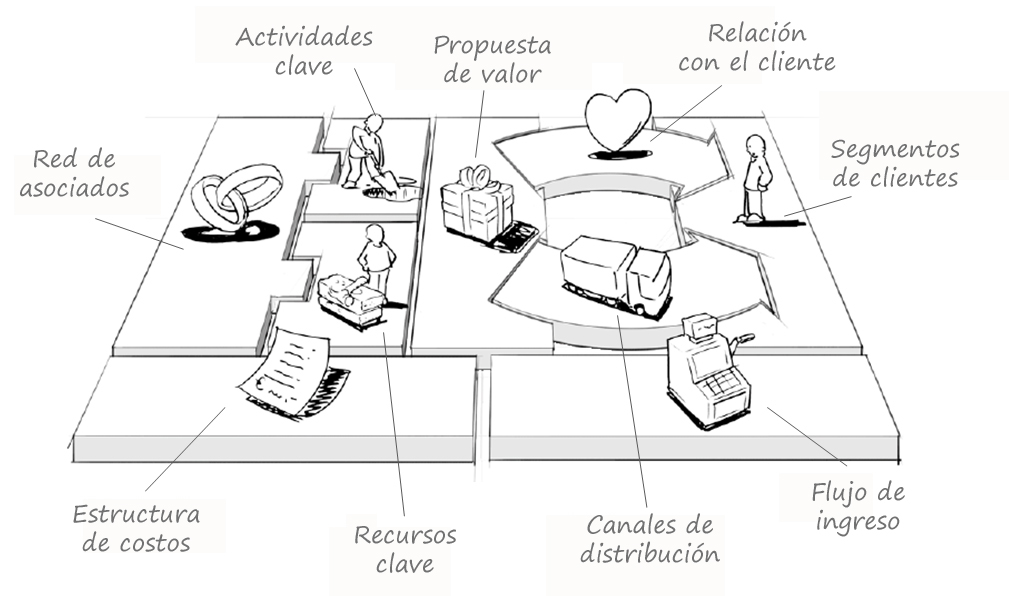
\includegraphics[width=0.8\linewidth]{figures/images/lienzo_modelos.jpg}
  \caption{Lienzo de modelos de negocio}
  \source{\url{https://www.educadictos.com/business-model-canvas/}}
  \label{fig:bmc}
\end{figure}